% main.tex
%
% (c) 2024 Lukas Schöpf, OST Ostschweizer Fachhochschule
%


\documentclass[hidelinks]{report}
% öffnet packages.tex
%
% packages.tex -- TeXfiles
%
% (c) 2023 Jakob Gierer & Lukas Schöpf, OST Ostschweizer Fachhochschule
%


%packages
\usepackage[english]{babel}
\usepackage[utf8]{inputenc}
\usepackage{csquotes}
\usepackage[T1]{fontenc}
\usepackage[backend=biber, style=ieee]{biblatex}
\usepackage{hyperref}
\usepackage{amsmath,amscd}
\usepackage{amssymb}
\usepackage{amsfonts}
\usepackage{amsthm}
\usepackage{amsmath}
\usepackage{makecell}
\usepackage{txfonts}
\usepackage{graphicx}
\usepackage{tabularx}
%\usepackage{subcaption}
\usepackage{subfig}
\usepackage[many]{tcolorbox}
\usepackage[acronym]{glossaries}
\usepackage{fancyhdr}
\usepackage[headheight=12.1pt]{geometry}
\usepackage[english]{cleveref}
\usepackage{lmodern}
\pagestyle{fancy}


%Für Test
%\usepackage{blindtext}


\addbibresource{references.bib}
\bibliography{references}
\makeglossaries
%
% acro.tex
%
% (c) 2024 Lukas Schöpf, OST Ostschweizer Fachhochschule
%
\newacronym{ost}{OST}{Ostschweizer Fachhochschule}
\newacronym{snr}{SNR}{Signal to Noise Ration}
\newacronym{cnn}{CNN}{Convolutional Neural Networks}
\newacronym{clip}{CLIP}{Contrastive Language-Image Pre-training}
\newacronym{align}{ALIGN}{A Large-scale ImagGe and Noisy-text embedding}
\newacronym{sam}{SAM}{Segment Anything}
\newacronym{hef}{HEF}{Hailo Executable File}
\newacronym{dfc}{DFC}{Dataflow Compiler}
\newacronym{pca}{PCA}{Principal Component Analysis}
\newacronym{har}{HAR}{Hailo Archive}
\newacronym{tse}{TSE}{Tiled Squeeze-and-Excite}


% name des tex-file Reinschteiben welches man bearbeitet
% Auskommentiern um ganzes Dokument zu setzen
%\includeonly{text/Entwicklung} 

\begin{document}
    \pagenumbering{Roman}
     % öffnet titlepage.tex
    %
% titlepage.tex -- TeXfiles
%
% (c) 2024 Jakob Gierer & Lukas Schöpf, OST Ostschweizer Fachhochschule
%


\begin{titlepage}
    % Bigger symmetric margins
    \newgeometry{
        outer = 3cm, inner = 3cm, top=5cm,bottom=6cm
    }
    \centering
%    \vspace{4cm}

    % Titel
    {\huge \bfseries \sffamily Scene Understanding \par
     \normalfont\itshape On-Site Scene Understanding with Edge AI \par}
    \vspace{1cm}

    % Autoren
    {\large \textsl{Lukas Schöpf}}
    \par
    \vspace{1cm}

    % Informationen über Hochschule
    {\textsc Master Project \par}
    {Ostschweizer Fachhochschule \par}
    \today
    \vfill
    
    % Titelbild
    % Beispiel
%    \begin{figure}[h]
%        \centering
%        \includegraphics[width=3cm]{example-image-c}
%    \end{figure}

    % Oder Tikz
    % \resizebox{.9\linewidth}{!}{
        %   \input{figures/tikz/}
        % }
    \vfill

    % Wichtige Informationen
    \begin{tabular}{rl}
        \bfseries\sffamily Advisor              & Prof. Andreas Breitenmoser \\
        \bfseries\sffamily Industry partner     & Hexagon AB \\
        \bfseries\sffamily Co-advisor Hexagon   & Martin Winistörfer \\
    \end{tabular}
    \restoregeometry    
\end{titlepage}


    %
% Abstract.tex
%
% (c) 2024 Lukas Schöpf, OST Ostschweizer Fachhochschule
%

\chapter*{Abstract}

	
	
    %%
% Dankessagung.tex
%
% (c) 2023 Jakob Gierer & Lukas Schöpf, OST Ostschweizer Fachhochschule
%

\chapter*{Danksagung}

Wir möchten diese Gelegenheit nutzen, um unseren aufrichtigen Dank all jenen auszudrücken, die uns während der Erstellung unserer Bachelorarbeit unterstützt und inspiriert haben.
\vspace{11pt}

\noindent
Ein besonderer Dank gilt auch unseren Betreuungspersonen, Patrik Müller und Hannes Badertscher.
Ihre fachliche Expertise, ihre Geduld und ihre Ratschläge waren von unschätzbarem Wert für den Erfolg unserer Arbeit.
Wir sind dankbar für die konstruktive Kritik und die Unterstützung, die sie uns entgegengebracht haben.
\vspace{11pt}

\noindent 
Ein herzliches Dankeschön geht auch an Florian Baumgartner und Alain Keller, die uns bei der Anpassung und Benutzung ihres Codes unterstützten. 
\vspace{11pt}

\noindent
Ausserdem möchten wir unseren Familien für das Korrekturlesen unserer Bachelorarbeit danken. 
    \pagestyle{plain}
    \tableofcontents
    {
    	\linespread{0.7}\selectfont{}
    	\glsnogroupskiptrue
    	\printglossary[type=\acronymtype]
    }
    % add common macros
    %
% macros.tex
%
% (c) 2023 Jakob Gierer & Lukas Schöpf, OST Ostschweizer Fachhochschule
%

% Kopfzeilen
%
\renewcommand{\headrulewidth}{0.4pt}
\renewcommand{\chaptermark}[1]{%
    \markboth{#1}{}
}
\renewcommand{\sectionmark}[1]{
    \markright{#1}
}

\rhead{\leftmark}
\lhead{\rightmark}

%to set Numbers in Circles use \kreis{}
\newcommand{\kreis}[1]{\unitlength1ex
    \begin{picture}(2.5,2.5)
        \put(0.75,0.75){\circle{2.5}}\put(0.75,0.75){\makebox(0,0){#1}}
\end{picture}}

%for different colored Text
\definecolor{YellowOrange}{RGB}{255, 159, 43}
\definecolor{RoyalBlue}{RGB}{0, 122, 255}
\definecolor{ForestGreen}{RGB}{18, 159, 87}

% Beispiel umgebung erstellen
\newcounter{satz}[chapter]
\newenvironment{beispiel}{%
    \refstepcounter{satz}
    \begin{proof}[Beispiel \arabic{chapter}.\arabic{satz}]%
        \renewcommand{\qedsymbol}{$\bigcirc$}
    }{\end{proof}}
    \newpage
    \pagenumbering{arabic}
    \pagestyle{fancy}
    % ==================================================
    % Beispiel um externe Textdokumente hinzuzufügen 
    % \input{file}
    \chapter{Introduction}
Hexagon AB\cite{hexagon} is a global player in digitisation technology and specializes in measurement and positioning systems.
Hexagon’s laser scanning devices produce point cloud data of the environment and capture images through additional cameras integrated into their scanners.
A challenge in Hexagon’s laser scanning applications is to build ever smarter scanning devices which have better understanding of the scenes they are placed in by preferably pre-processing the environment
information they record directly in the field.

The goal of this project is to work towards integration of enhanced scene understanding capabilities into the scanning application’s edge devices.
A scanner should, for example, be able to classify a scene on various hierarchical levels and with increasing level of detail, namely indoor vs. outdoor, construction site 
vs. completed building (eventually inferring even the degree of building completion), office complex vs.
family house, small vs. big room, kitchen vs. bathroom, bathroom with vs. without bathtub, etc.

To this end, this project aims at evaluation, implementation, and test of smaller machine learning models
suitable for an Edge AI platform to demonstrate that corresponding classification tasks
could be embedded on board of a laser scanner in the future.
    \chapter{Task}
This work shall include the following work packages:
\subsection*{State-of-the-art in Scene understanding}
\begin{itemize}
    \item Get familiar with the state-of-the-art concerning machine learning/deep learning models for environment recognition and scene understanding by reading the relevant scientific papers, covering foundation models like SAM\cite{sam} or CLIP \cite{clip}.
    \item Understand the working principles of existing approaches, especially CLIP and TinyCLIP\cite{tinyclip}, in detail.
    \item Gather experience with CLIP-based models by experimenting on suitable available datasets and code (openly available or provided by Hexagon) within a PC-environment (e.g., Python-based application). The dataset provided by Hexagon provides over 1000 panoramic images from at least five different classes.
\end{itemize}

\subsection*{Hardware accelerator Overview}
\begin{itemize}
    \item Perform a brief market analysis to collect an updated view of currently active players (universities, startups, and larger companies) for the provision of AI hardware accelerators with M.2 interface capabilities (like the one of Raspberry Pi AI Kit), which could be effectively used for a CLIP-based approach like in our project.
    \item Set up the Raspberry Pi AI Kit and its toolchain, and specifically compare the Hailo AI accelerator with the other hardware accelerators found from above.
\end{itemize}

\subsection*{CLIP model on Edge AI Platform}
\begin{itemize}
    \item Integrate a state-of-the-art machine learning algorithm like TinyCLIP on Raspberry Pi AI Kit (typically using Python on Raspberry Pi and C/C++ for Hailo AI accelerator).
    \item Test the performance of the implementation (using meaningful metrics) and run benchmarking to evaluate differences (e.g., in performance) when computing CLIP in the cloud vs. on the edge.
    \item Create a proof-of-concept with the Raspberry Pi AI Kit platform that demonstrates feasibility of the use case by processing realistic datasets from Hexagon.
\end{itemize}

\subsection*{Enhanced Proof-of-Concept}
\begin{itemize}
    \item Add some own improvements regarding performance, reliability, or generalization to the existing AI models and/or platform ports, considering quantization, pruning, architecture modifications, dataset processing, training, and optimized hardware deployments (allocation).
    \item Generalize the implementation to arrive at a unified Edge AI platform framework that can operate with ideally any other AI hardware accelerator card providing a M.2 slot interface.
    \item \textit{Optionally} Expand the used machine learning pipeline to support multi-label classification.
    \item \textit{Optionally}  Extend the given framework and platform to test other foundation models (like SAM) in an edge deployment.
    \item \textit{Optionally}  Explore the possibility to incorporate user feedback and a respective feedback mechanism on the platform, which may offer valuable continuous updates in an effort towards online learning.
\end{itemize}
    \chapter{Literature research}

This Literature research studied relevant papers in the field of scene understanding.
State of the art is to use deep learning models for scene understanding tasks.
The goal of to discover the semantic information whthin a given scene, which is the base for many applicaitions such as surveillance, autonomous driving, traffic savety, vision-guided mobile navigation and many more.
The term gains a lot of relevantcy because of the rapid evolution of neural networks over the last couple years.
Most of the papers found online tackel the topic of autonomous driving\cite{sceneunderstandingautdriving1}.
In early research \acrfull{cnn}\cite{SegNet} were mostly used for this task.
With the introduction of the transformer \cite{attentionisallyouneed} many researchers moved on to this new arcitecture.
Soon multi-modal networks like CLIP\cite{clip} and ALIGN\cite{ALIGN} came up.
These networks use a text- and image-encoder to learn an predict relations between image and text pairs.


    %
% clip.tex
%
% (c) 2024 Lukas Schöpf, OST Ostschweizer Fachhochschule
%

% DeepL corrected
% explain Resnet and transformer

\chapter{Cross-modal networks
    \label{chapter:crossmodalnetworks}}
    Multimodal deep learning is the study of models that learn from multiple modalities. 
    For example, humans can use both vision and hearing to identify an object or a person. 
    Cross-modal deep learning leverages data from one modality to improve performance in another. 
    For instance, if a person looks at a picture of a bird and listens to its song, they might be able to identify the bird more effectively.

    One of its most impressive features is the ability to perform well on data the model has not been explicitly trained on. 
    This ability is known as zero-shot capability, which stems from N-shot capability. 
    N-shot capability refers to the number of training samples of a particular class that a model needs to classify it correctly.

    In this work, cross-modal networks are used to identify relationships between images and text. 
    Most cross-modal networks designed for this task consist of a text encoder and an image encoder.

    \section{Base Networks}
    To understand cross-modal networks, it is essential to first examine their components. 
    Most of these networks employ transformers as encoders, although some utilize ResNets. 
    The information presented in this section is derived from the corresponding paper and \cite{clipexplain}.

    \subsection{ResNet
    \label{crossmodalnetworks:sec:resnet}}

    Residual Networks (ResNets) were introduced in \cite{resnetpaper}. 
    A ResNet employs residual blocks (\cref{fig:crossmodalnetworks:resblock}), which incorporate residual connections between certain layers. 
    These connections allow information to bypass specific layers, facilitating the training of deeper networks by mitigating issues such as the vanishing gradient problem. 
    This mechanism stabilizes the training process and accelerates the convergence of deep neural networks. 
    The primary motivation for ResNets was to enhance image processing capabilities beyond those of traditional \acrfull{cnn}s. 
    Notably, large transformer models, such as OpenAI's GPT series, also utilize residual connections to improve performance and enable the training of deeper architectures \cite{attentionisallyouneed}.
    
    \begin{figure}[h]
        \centering
        \includegraphics[width=0.55\textwidth]{Images/crossmodalnetworks/ResBlock.png}
        \caption{Image of a ResNet block.\cite{resnetpaper}}
        \label{fig:crossmodalnetworks:resblock}
    \end{figure}

    \subsection{Transformer}

    The Transformer was first introduced in \cite{attentionisallyouneed}.
    Most of the information in this section is derived from that paper. 
    Before Transformers, \acrfull{rnn}s were commonly used to process sequential data. 
    To capture dependencies and relationships within an input sequence, a mechanism called attention was introduced.
    The Transformer marked a significant breakthrough by introducing a mechanism known as self-attention.
    Self-attention does not need to be calculated sequentially.
    It is defined as:

    \begin{equation}
        \text{Attention}(Q, K, V) = \text{softmax}\left(\frac{QK^T}{\sqrt{d_k}}\right)V
        \label{equ:selfattention}
    \end{equation}

    where \(Q = XW_q\), \(K = XW_k\), and \(V = XW_v\). 
    Here, \(X\) represents the input, and \(W_{q}\), \(W_{k}\), and \(W_{v}\) are learnable parameter matrices. 
    The matrices \(Q\), \(K\), and \(V\) are referred to as query, key, and value, respectively. 
    The term \(\frac{1}{\sqrt{d_k}}\) is a scaling factor to normalize the output, where \(d_k\) is the dimensionality of the key vectors.
    
    Often, multiple attention heads are used simultaneously to allow the model to focus on different parts of the input sequence (see \cref{fig:crossmodalnetworks:attention}).
    
    \begin{figure}[]
        \centering
        \includegraphics[width=0.7\textwidth]{Images/crossmodalnetworks/attention.png}
        \caption{Single and multi-head attention\cite{attentionisallyouneed}}
        \label{fig:crossmodalnetworks:attention}
    \end{figure}

    With the introduction of the self-attention mechanism, the need for \acrshort{rnn}s became obsolete. 
    \acrshort{rnn}s are challenging to train due to issues such as the vanishing or exploding gradient problem. 
    Additionally, they are difficult to parallelize because of their sequential nature. 
    These issues no longer occur when using a Transformer, as it processes sequences in parallel and effectively captures long-range dependencies.


    \begin{figure}[]
        \centering
        \includegraphics[width=0.25\textwidth]{Images/crossmodalnetworks/The-Transformer-encoder-structure.png}
        \caption{Image of a Transformer which in the case of CLIP is used as a text encoder\cite{attentionisallyouneed}}
        \label{fig:crossmodalnetworks:transformer}
    \end{figure}

    To use a Transformer, the input must first be split into tokens. 
    These tokens represent text snippets in the case of a text Transformer or patches of an image in the case of a Vision Transformer (ViT) (see \cref{fig:crossmodalnetworks:visiontransformer}). 
    These tokens or patches are then embedded into a high-dimensional vector space. 
    For example, in the case of the CLIP ViT-32 visual encoder, each vector has 1024 dimensions.

    Additionally, positional embeddings are added to the token embeddings to retain information about the order or spatial arrangement of the tokens. 
    Next, a combination of self-attention blocks and feed-forward layers is used to process the tokens (see \cref{fig:crossmodalnetworks:transformer}). 
    Residual connections and normalization are also employed to facilitate training.
    Multiple such blocks are concatenated to form the full Transformer architecture.

    \begin{figure}[]
        \centering
        \includegraphics[width=0.6\textwidth]{Images/crossmodalnetworks/Vision_Transformer.png}
        \caption{Vision Transformer architecture\cite{vitwikipedia}}
        \label{fig:crossmodalnetworks:visiontransformer}
    \end{figure}

    \section{Text Encoder}

    The text encoder is typically implemented as a Transformer. 
    Its purpose is to encode a given text into a high-dimensional vector space. 
    This vector space enables the encoder to classify unseen classes by placing their vectors close to those of related classes. 
    In theory, the closer two words are related, the closer their corresponding embedding vectors are in the high-dimensional space.

    An example of this relationship can be visualized in \cref{fig:crossmodalnetworks:3demb}, where \acrfull{pca} is used to reduce the dimensionality of the embedding vectors. 
    For instance, the words "cat" and "dog" appear close together because they share a semantic relationship.

    \begin{figure}
        \centering
        \includegraphics[width = 0.8\textwidth]{Images/crossmodalnetworks/3DEmbedding.png}
        \caption{Example of text embedding using CLIP and \Acrshort{pca}}
        \label{fig:crossmodalnetworks:3demb}
    \end{figure}
    
    \section{Image encoder}

    In most cases, the image encoder consists of a Vision Transformer \cite{Vis_N_Grams}. 
    Like the text encoder, the image encoder transforms an image into a high-dimensional vector space. 
    A Vision Transformer requires the input image to have a specific dimension. 
    For this reason, an image encoder typically consists of a Vision Transformer and a preprocessor, which transforms the image into the correct dimensions for the Vision Transformer.

    \section{Contrastive Language-Image models
        \label{section:languageimagemodels}}
        This section explores models that use both text and image modalities. 
        Most of the information in this section is derived from \cite{cliplikeweb} and related papers.

        Contrastive techniques involve paired inputs from two modalities (e.g., an image and its corresponding caption). 
        Each input is embedded into its own embedding space. 
        The goal is for such pairs to be represented in similar embeddings by their respective encoders. 
        The term "language-image" refers to the two modalities used by the model. 
        Most of these models are pre-trained on large, general datasets. 
        Pre-training means that the model has been trained on a broad, universal dataset. 
        For a specific application, a pre-trained model can be fine-tuned to improve its performance on the targeted task.

        \subsection{CLIP
            \label{section:clip}}
        \acrfull{clip} \cite{clip} is a cross-modal model developed by OpenAI \cite{openai} that evaluates how well a given image and text match. 
        It can be used with various image and text encoders. 
        The model is trained on a large dataset consisting of 400 million image-text pairs. 
        \acrshort{clip} has been shown to outperform some of the best-known models in image classification. 
        Many other models build upon \acrshort{clip} as a foundation, improving upon it to create more advanced architectures.
            

        \begin{figure}[]
            \centering
            \includegraphics[width=\textwidth]{Images/crossmodalnetworks/OpenAICLIP.png}
            \caption{A picture from the \acrshort{clip} paper by OpenAI \cite{clip}.}
            \label{fig:crossmodalnetworks:openaiclip}
        \end{figure}

        \subsection{ALIGN
            \label{section:align}}
        \acrfull{align} \cite{ALIGN} was released shortly after \acrshort{clip}. 
        Rather than relying on small image-caption datasets, \acrshort{align} uses a dataset of 1.8 billion image-alt-text pairs (e.g., as shown in \cref{fig:crossmodalnetworks:alignepairs}). 
        These alt-text descriptions are much noisier than captions. 
        The authors apply basic filtering techniques to remove duplicates, images with more than 1000 associated alt-texts, and uninformative alt-texts (such as those that are either too frequent or contain rare tokens), while avoiding expensive filtering operations. 
        With these simple steps, \acrshort{align} meets or exceeds the state-of-the-art performance on several zero-shot and fine-tuning tasks.
            
        \begin{figure}
            \centering
            \includegraphics[width=\textwidth]{Images/crossmodalnetworks/examplepicsalign.png}
            \caption{Example of alt-text image pairs from the train dataset from \acrshort{align}\cite{ALIGN}}
            \label{fig:crossmodalnetworks:alignepairs}
        \end{figure}

        In a test described in this paper, \acrshort{align} was much slower than \acrshort{clip} when performing a zero-shot evaluation on the CIFAR100 \cite{cifar100} dataset. 
        For a single prediction, \acrshort{align} takes 70 times longer than \acrshort{clip} (see \cref{tab:clipaligntest}). 
        Neither of the networks were fine-tuned, and the highest predicted label was used. 
        Due to the slow inference speed, ALIGN was stopped after processing 35\% of the dataset.

        \begin{table}
            \centering
            \begin{tabular}{lll}
                \hline
            \textbf{Measurment}&\textbf{ALIGN}&\textbf{CLIP}\\\hline
            Accuracy& 48.9\% & 61.7\%\\
            Speed(seconds per iterarion)&  2.16&  0.02\\ \hline
            \end{tabular}
            \caption{First test on CIFAR100.}
            \label{tab:clipaligntest}
        \end{table}

        \subsection{TinyCLIP
            \label{section:tinyclip}}
        \begin{figure}
            \centering
            \includegraphics[width=\textwidth]{Images/crossmodalnetworks/TinyCLIP.jpg}
            \caption{Optimization which are used in TinyCLIP\cite{tinyclip}}
            \label{fig:crossmodalnetworks:tinyclip}
        \end{figure}

        TinyCLIP \cite{tinyclip} is a cross-modal distillation method designed for large-scale pre-trained speech-image models. 
        TinyCLIP can be used on resource-limited systems due to its miniaturization. 
        It also accelerates training with minimal loss in model accuracy. 
        The method utilizes three key concepts to reduce the size of the network.


        \subsubsection{Affinity mimicking}
        Affinity mimicking is a specialized form of knowledge distillation, also known as model distillation. 
        In knowledge distillation, a larger teacher network is trained first. 
        After training the teacher network, a smaller student network is trained to predict the output of the teacher network. 
        This approach works because the output of the teacher network contains more information than the original label. 
        Affinity mimicking introduces two new metrics in the training process: language-to-image loss and image-to-language loss (\(L_{t2i}\) and \(L_{i2t}\), as shown in \cref{fig:crossmodalnetworks:tinyclip}).


        \subsubsection{Weight inhertiance
        \label{section:weightinheritance}}
        Weight inheritance is a technique that transfers important weights from well-trained teacher models to smaller student models. 
        In the paper, the authors propose two methods:
        \begin{itemize}
            \item \textbf{Manual weight inhertiance:} Based on the authors' observations, text encoders exhibit the most redundancy in depth (layer-wise), while image encoders exhibit redundancy in width (channel-wise). 
            They select \(k\) layers and channels from a branch to serve as initialization weights. 
            To select the most important weights, some prior knowledge is required.
            \item \textbf{Automatic weight inhertiance:} The authors introduce a learnable mask to determine the importance of each weight.
        \end{itemize}

        \subsubsection{Multi-stage progressiv distillaiton}
        The model is pruned in several steps. 
        At each stage, the authors apply a modest degree of compression (e.g., 25\%). Each stage also includes weight inheritance and affinity mimicking.
        

\section{Enhance the algorithm
    \label{section:enhancealgorithm}}

    To improve the accuracy of a pre-trained network, it can be fine-tuned for a specific task. 
    Fine-tuning is a broad term, encompassing methods ranging from the simple addition of a learnable linear layer at the end of the network to feature distillation. 
    The concept of fine-tuning is derived from transfer learning \cite{transferlearning}, where the final layers of a neural network are removed and the network is retrained with new, independent layers. 
    This approach saves time and resources. 
    For example, in CLIP, a linear layer can be added to enhance classification performance \cite{finetuneclip}. 
    All fine-tuning approaches rely on the output of the network for further processing. 
    Another way to increase accuracy is by using better-fitting text prompts.
    
\section{Conclusion multi-modal networks}
    Based on the results of our own testing, ALIGN is not considered a suitable solution for this work. 
    Instead, the focus is on CLIP and TinyCLIP, which can be fine-tuned to further improve their performance. 
    Additionally, the performance of these models can be enhanced by using more effective text prompts.
    \chapter{Market analysis}

% Write More and display table somewhere

A part of this work is a market analysis of the available hardware accelerator with M.2 interferance.
The found accelerator are summerised in table.
Many of the available product are either to old and weak (Coral M.2 accelerator) or only available as preorder.
From the current lookt at products, Hailo seems as the most suited for this project.
It uses less power than products from Coral with higher TOPS.

For the future a hradware accelerator which has the capability to process floating point models looks very intressting.
But the advantage from floating point to intger has to be proven.

There are also many suppliers which produce accelerator chips.
It is possible to design a PCB with an M.2 slot yourself to be less dependend on supplier software.


% \begin{table}
%     \centering
%     \begin{tabular}{|l|l|l|r|r|l|}
%     \hline
%         \thead{Product Name }& \thead{Manufacturer} & Availability & \makecell{Processing \\Power \\(TOPS INT8)} & \makecell{Processing\\ Power\\ (TFLOPS BF16)} & \makecell{Power\\ Consumption} \\ \hline
%         Hailo-8L Entry-Level M.2 Module & Hailo & Available & 13 & ~ & 1.5 W \\ \hline
%         Hailo-8 M.2 AI Acceleration Module & Hailo & Available & 26 & ~ & 2.5W \\ \hline
%         Metis M.2 Card & Axelera & Preorder & 214 & ~ & 4-8 W \\ \hline
%         SAKURA-II M.2 & Edge Cortix & Preorder & 60 & 30  & 10 W \\ \hline
%         M.2 Accelerator & Coral & Available & 4 & ~ & 2 W \\ \hline
%         M.2 Accelerator Dual Edge TPU & Coral & Available & 8 & ~ & 4 W \\ \hline
%         ME1076 M.2 Accelerator Card & Mythic & ~ & 25 & ~ & 3.5 W \\ \hline
%         MM1076 M.2 Accelerator Card & Mythic & ~ & 25 & ~ & 3.5 W \\ \hline
%         MLSoC Dual M.2 Production Board & Sima.ai & ~ & 50 & ~ & 15 W \\ \hline
%         Orca 1.1 M.2 & DeGirum & In Stock & ~ & ~ & ~ \\ \hline
%     \end{tabular}
% \end{table}
    \chapter{Hardware Accelerator}

The Raspberry Pi 5 with an AI kit was chosen as the hardware to demonstrate the concept of edge computing.  
This decision was made based on recommendations from the advisors and the availability of the hardware.  
The market analysis confirms this choice.  
The hardware accelerator in the AI kit is produced by Hailo \cite{hailo}.  

Generally, a hardware accelerator is used to compute neural networks, similar to how a GPU is used for graphics processing.  
Hailo is a company that produces hardware accelerators.  
The AI kit uses the Hailo-8L entry-level accelerator.  
Hailo provides a pipeline to compile a network for execution on their hardware.  

First, we will examine the network compilation process, which must be done on a PC, preferably one with a GPU.  
Then, we will look at how to run the network on the edge.  

\section{Network Compilation}

As mentioned before, the network has to be precompiled on a PC.  
The application designed for this task is called the \Acrfull{dfc}.  

\subsection{Dataflow Compiler  
\label{section:dfc}}  
Information and images are taken from the Hailo Dataflow Compiler User Guide \cite{hailo_dataflow_compiler}. 
To use the \acrshort{dfc}, a PyTorch or TensorFlow model must be converted to ONNX or TensorFlow Lite.   
The \acrshort{dfc} then compiles the model to a \Acrfull{hef} by executing the following steps:  

\begin{enumerate}
    \item Full Precision Optimization
    \item Quantization Optimization
    \item Compilation
\end{enumerate}

In the full precision optimization step, the ONNX file is first compiled into a \acrfull{har} file, a file type defined by Hailo.  
This step also can include changes to the model in the floating-point precision domain, such as Equalization \cite{meller2019same}, \acrshort{tse} \cite{Vosco_2021_ICCV}, and pruning.  

In the quantization optimization step, the model is compressed.  
This means that the model is converted from floating-point to integer.  
Weights are compiled to either 4, 8, or 16 bits, while activations are compiled to 8 or 16 bits.  
Which quantization is applied is handled through a model script.  
In that script, the amount of quantized weights can be specified.  
It is also possible to target specific layers through the model script.  
Additionally, preprocessing steps can be added to the model script, such as resizing the input or converting the input from RGB to YUV.  

The result of this step is a quantized \acrshort{har} file.  
This file can then be compiled into a \acrshort{hef} file for use on Hailo hardware.  

\begin{figure}[]
    \centering
    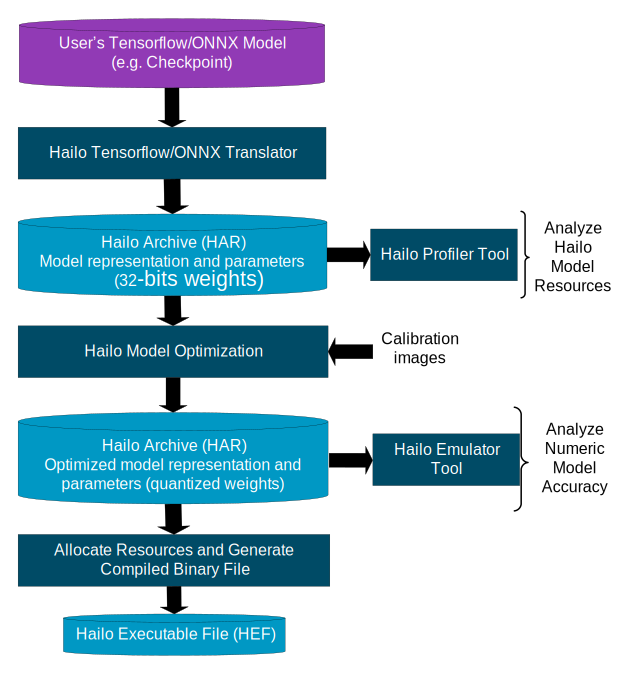
\includegraphics[width=0.8\textwidth]{Images/Hardware/model_build_overview_with_onnx_and_hef_w_har.png}
    \caption{\Acrlong{dfc} overview \cite{hailo_dataflow_compiler}}
    \label{fig:hardware:dfcoverview}
\end{figure}

\subsection{Constraints}
At the time of this writing, the \acrshort{dfc} is not capable of compiling Transformers.  
This is an important limiting factor for this project.  
The best performance for CLIP is achieved with Vision Transformers as the image encoder.  
Fortunately, the visual encoding of CLIP can also be performed with ResNet (see \cref{crossmodalnetworks:sec:resnet}).  

\section{Running on the Edge}

Hailo provides a library called TAPPAS, which is based on GStreamer.  
This library enables the use of a Hailo device within GStreamer pipelines to create intelligent video processing applications.  
The information for this section is taken from the TAPPAS User Guide.  

At present, there are two approaches to run a network on a Hailo device:  
one using GStreamer and another using a Python API.  
There are many different example applications available for various use cases.  
These examples can be found in the Hailo Model Zoo \cite{hailo_model_zoo} or in their repository for Raspberry Pi examples \cite{hailo_rpi5_examples} or general application code examples \cite{hailo_application_code_examples}.  

\subsection{GStreamer Approach}

GStreamer is a framework for creating streaming media applications.  
It enables the design of any type of multimedia application, but it is not restricted to audio and video processing.  
The framework can process any kind of data flow.  

GStreamer consists of blocks that can be concatenated.  
To work with the Hailo hardware accelerator, some blocks in the pipeline are offloaded to the Hailo processor.  
A Python program is used to construct a string, which is then executed in a terminal.  
An example pipeline can be seen in \cref{fig:hardware:gstreamerpipeline}.  
More examples with code can be found in the TAPPAS User Guide.

\begin{figure}[]
    \centering
    \includegraphics[width=\textwidth]{Images/Hardware/gstreamerExample.png}
    \caption{Example GStreamer pipeline from TAPPAS User Guide}
    \label{fig:hardware:gstreamerpipeline}
\end{figure}

\subsection{Python API Approach}

With the Python API approach, one can execute the entire inference in Python.  
This makes the program much simpler compared to the GStreamer approach.  
In Python, the Hailo hardware accelerator is treated as an object with dedicated functions for inference.  
It is important to note that Hailo swaps the input dimensions of the network.  
This means that the dimensions of the input to the network must be adjusted accordingly.  
Due to the complexity of the GStreamer approach, the Python API is used in this project.
    \chapter{System Overview}

The goal of the system is to classify panorama images into defined classes.
For that a CLIP like network is used on the edge.
As a computing platform a Raspberry Pi 5 with the hardware accelerator extension is used.
The hardware Accelerator is the Hailo-8L entry level accelerator (\cref{fig:overview:aikit}).
The System which is used and developt in this work, can be divided in 2 parts.
One part is the compilation of a neural network on a PC.
The other part is the inference of a compiled network on the Raspberry Pi.

\begin{figure}[h]
    \centering
    \includegraphics[width=0.5\textwidth]{Images/SystemOverview/ai-kit.png}
    \caption{Picture of the hardware accelerator mounted on a Raspberry Pi 5\cite{bildAiKit}}
    \label{fig:overview:aikit}
\end{figure}



\section{Compilation of a Network}

\begin{figure}
    \centering
    \includegraphics[width=\textwidth]{Images/SystemOverview/DFCFlow.pdf}
    \caption{Visualisation of the compilation work flow}
    \label{fig:overview:dfcflow}
\end{figure}
First the image encoder either from \acrshort{clip} or TinyCLIP has to be aquuired.
This encoder then gets exported as a ONNX graph.
The part from the graph which doesn't compile gets cut of and saved for later.
Then the edited graph gets compiled.
During compilation, the network is quantized and simplified.
This reduces the amount of memory and processing power needed to use a network.
The network has to be compiled to format which can be executed on the hardware accelerator.
In this work the compilation is done with the \Acrlong{dfc} (see \cref{section:dfc}) from Hailo.
The result is a \acrshort{hef} file which can be executed on hailo hardware.

\section{Inference on Raspberry Pi}

\begin{figure}
    \centering
    \includegraphics[width=\textwidth]{Images/SystemOverview/Overview.drawio.pdf}
    \caption{System work flow}
    \label{fig:overview:overview}
\end{figure}

To use a network on a hardware accelerator a specific software has to be used.
Because of current limitations of the \acrshort{dfc}, self attention layers were unable to compile.
Because of this constraint the text encoder of CLIP must be executed in advance on an PC.
The resulting text embeddings then get loaded on to the Raspberry Pi in form of a json file.
The constrain also doesnt allow transformers to compile.
Because of that reason ResNets were used as image encoders.
The problem with the resnets was, that the last layer also is a self attention layer.
To get the network to compile, the last part got cut off and is later processed as a from of postprocessing.


    \chapter{Hexagon Dataset}
The dataset was collected using the terrestrial laser scanner RTC 360 from Leica at 32
different locations.
In total, this dataset consists of 1330 images and the number of images per location ranges from 4 to 423.
All the images are 360-degree panoramas with a
resolution of 8192 \(\times\) 4096 pixels.
The images are divided into the following 5 classes:
\begin{itemize}
    \item Indoor architectural
    \item Indoor construction
    \item Outdoor construction
    \item Outdoor Urban
    \item Forest
\end{itemize}



\begin{table}[htbp]
    \centering
    \begin{tabular}{ccc}
    \toprule
    \textbf{1. Original}& \textbf{2. Rephrased}& \textbf{3. Subclasses}\\ \midrule
    Construction (in) & construction site & \makecell{construction site,\\ mining, tunnel}\\ \hline
    Architectural (in)& architectural& \makecell{architectural, office,\\ residential, school,\\ manufacturing, cellar,\\ laboratory} \\ \hline
    Construction (out)& construction site & construction site \\ \hline
    Urban (out)& town & \makecell{town, city,\\countryside, alley,\\ parking lot} \\ \hline
    Forest (out)& forest& forest \\
    \bottomrule
    \end{tabular}
    \caption{Rephrased terms and their subclasses}
\end{table}
    \chapter{Implementation
    \label{chapter:implementation}}

This chapter discribs the tools, methods and reasons for the from of implementation.
As sad due to early test CLIP and TinyCLIP are used as models.

\section{Model acquisition}

The CLIP models are taken from the official CLIP Github repo \cite{clipgit}.
The TinyCLIP models are taken from the official TinyCLIP Github repo \cite{tinyclipgit}.
There is also the posibility to take models from HuggingFace \cite{huggingface}.
The problem with HuggingFace is that the model cant be split into image and text encoder.
Because of this reason only models from the offical CLIP respectiv TinyCLIP repo were used.
In \cref{tab:methods:clipsize} one can see the parameter count for all CLIP and TinyCLIP implementation which use a ResNet as a visual encoder.
We see that TinyCLIP 
\begin{table}[h]
    \centering
    \begin{tabular}{lll}
    \hline
    Model name & \begin{tabular}[c]{@{}l@{}}Parameters\\ Visual(Mio)\end{tabular} & \begin{tabular}[c]{@{}l@{}}Parameters\\ Text(Mio)\end{tabular} \\ \hline
    RN50                & 38  & 38  \\
    RN50x4              & 87  & 59  \\
    RN50x16             & 167 & 850 \\
    RN50x64             & 420 & 151 \\
    RN101               & 56  & 38  \\
    TinyCLIP-ResNet-19M & 19  & 19  \\
    TinyCLIP-ResNet-30M & 30  & 29  \\ \hline
    \end{tabular}
    \caption{Paramter count for different CLIP implementations with ResNet as visual encoder}
    \label{tab:methods:clipsize}
\end{table}

\section{Model translation}
The models were first split into image and text encoder.
The image encoder then gets translated to a onnx graph and afterwards simplified.
This onnx graph then is translated by the \acrshort{dfc} to \acrshort{har} and \acrshort{hef} files.

\begin{figure}
    \centering
    \subfloat[End of CLIP ResNet50x4 vision encoder Onnx graph acquired though official CLIP]{\includegraphics[width=0.4\textwidth]{Images/Implementation/ClipRes50x4.png}\label{fig:implementation:clipres50x4}}
    \qquad
    \subfloat[End of CLIP ResNet 50x4 vision encoder Onnx graph sendt by Hailo]{\includegraphics[width=0.4\textwidth]{Images/Implementation/HailoClipRes50x4.png}\label{fig:implementation:hailoclipres50x4}}
    \caption{Comparison of CLIP ResNet 50x4 vision encoder Onnx graph (a) from official CLIP and (b) from Hailo}
    \label{fig:implementation:compareRN50x4}
\end{figure}

In that step lays the first big problem of the project.
As described in \cref{section:dfc} the \acrshort{dfc} is unable to compile transformers.
To be precise, a transpose block at the end of every self attention layer is were the problems lay.
The \acrshort{dfc} swaps dimensions and takes together the last 2 dimensions.
In the ResNet which is acquired though the offical code (see \cref{fig:implementation:clipres50x4}) one can see that the transpose block after the MatMul block swaps a second and the third dimension.
This leads to a compilation error because the \acrshort{dfc} already combined the last 2 dimensions.
This error does not occure when the model given by Hailo is compiled.
In \cref{fig:implementation:hailoclipres50x4} the maximum of dimensions is 3.

To work around this problem the last part of the onnx graph is cut off.
To cut the graph Onnx-Modifier \cite{onnxmodifier} is used.
The cut off blocks are implemented as postprocessing.
As described in \cref{section:dfc} a script can be applied to change the behavior of the \acrshort{dfc}.
% Add scripts

After quantisation the graph can again be visualized with a tool name profiler from hailo.
In \cref{fig:implementation:compareRN50x4qunathar} the compiled model with the cutoff end is visualized.
In this figure the combination of the last dimensions can be seen.

\begin{figure}
    \centering
    \includegraphics[width=0.4\textwidth]{Images/Implementation/ClipRes50x4_qunat_Har.png}
    \caption{Output of the \acrshort{dfc} from compiling the modified onnx graph of the ResNet50x4.}
    \label{fig:implementation:compareRN50x4qunathar}
\end{figure}

This graph then gets compiled to a \acrshort{hef} file which can be executed on Hailo hardware.
To use CLIP the text embeddings are also needed.
Due to the limitation that no transformers can be used with hailo the embeddings get calculated on a PC and the saved in a Json file.

\textbf{Comparison size}


\subsection{Pre-processing}

The hexagon dataset which is used as refrence consists of panorama pictures.
These pictuers get cut into 5 equal sized patches.
Every patch gets processed with CLIP.
To finally classify a image a mayority vote is taken over the subclasses of the patches.
This process is mentiond in Lia Winkler's report and increases the accuracy of the model.

\subsection{Post-processing}

As sad the cut of part of the Onnx graph is processed in post processing.
The Cut of part consists of one matrix multipication and some rearanging of the dimensions.
In a first implementation the weights for the matrix multipication were extracted and saved in a json file.
In a second attemp the cut off Onnx Graph is directly used.
The second attemp proved as faster while using much less memory.

\section{Inference}
To have a good comparison of performance the implementation on the Raspberry Pi is mostly similar to the one which is used on PC.
The PC application is mostly the same as Lia Winkler used in her work.
For Vision encoder only ResNet's were used because of the limitations from the \acrshort{dfc}.
The Hexagon dataset is used as image input.
As text input the subclasses from \cref{tab:dataset:subclasses} are used.
The text input were used solo or in a scentens.
In \cite{clip} the authors state that the performance of the network can improve if the text inputs are in a scentens.
To use the vision model on Hailo the python api is used.
2 diffrent implmentations were tested.
One proved much slower because the device initialisation happens every time a image is encoded.


To check the functionalit of the \acrshort{dfc} as test picture is used.
The \acrshort{dfc} is able to calculate the output of the compiling network at every step.
This is used to compare the output of the different stages with a test image.
The Results can be seen in \cref{tab:methods:clipcompare}.

\begin{table}[]
    \centering
    \begin{tabular}{llllll}
    \hline
    Labels        & a Human & a Cat   & a Dog  & a white cat & a small dog \\ \hline
    Original      & 1.57 \%  & 90.65 \% & 0.34 \% & 7.23 \%      & 0.2 \%       \\
    Nativ \acrshort{har}        & 1.57 \%  & 90.65 \% & 0.34 \% & 7.23 \%      & 0.2 \%       \\
    Compiled \acrshort{har}     & 1.57 \%  & 90.65 \% & 0.34 \% & 7.23 \%      & 0.2 \%       \\
    Qunatized \acrshort{har}    & 1.9 \%   & 90.10 \% & 3.49 \% & 3.63 \%      & 0.8 \%       \\ \hline
    \end{tabular}
    \caption{Output probabilitys of test image at diffrent \acrshort{dfc} stages with CLIP RN50x4 as image encoder}
    \label{tab:methods:clipcompare}
\end{table}

\begin{table}
    \centering
    \begin{tabular}{llllll}
    \hline
    Labels        & a Human & a Cat & a Dog & a white cat & a small dog \\ \hline
    Original      &         &       &       &             &             \\
    Nativ \acrshort{har}     &         &       &       &             &             \\
    Compiled HAR  &         &       &       &             &             \\
    Qunatized HAR &         &       &       &             &                   
    \end{tabular}
    \caption{Output probabilitys of test image at diffrent \acrshort{dfc} stages
    \label{tab:methods:tinyclipcompare}}
\end{table}

As suspected the accuracy reduces significant after quantisation.


\section{Measurments}

To measure the performance of the Hailo hardware the models were tested in 3 ways:
\begin{itemize}
    \item CPU PC
    \item CPU Raspberry Pi
    \item Hailo hardware accelerator
\end{itemize}

As values to measure the following found usefull:
\begin{itemize}
    \item Throughput(speed)
    \item Mermory(size)
    \item Accuracy
\end{itemize}
The implementations were made as similiar as possible to ensuer the values are correct. 

% classes = ["construction site", "town", "city",
% "country side", "alley", "parking lot", "forest"]

% === CLIP PC ===
% Label probs: tensor([[0.1811, 0.0591, 0.0398, 0.0643, 0.5045, 0.0731, 0.0782]])

% === CLIP ONNX ===
% Label probs: tensor([[0.1811, 0.0591, 0.0398, 0.0643, 0.5045, 0.0731, 0.0782]])

% === CLIP HAR Nativ ===
% Label probs: [[0.18112072348594666, 0.05905136093497276, 0.03980713337659836, 0.06425424665212631, 0.5045444965362549, 0.07307031750679016, 0.07815175503492355]]

% === CLIP HAR Compiled ===
% Label probs: [[0.1811216175556183, 0.05905177444219589, 0.03980710357427597, 0.06425445526838303, 0.5045422315597534, 0.07307054847478867, 0.07815229147672653]]

% === CLIP HAR Quantized ===
% Label probs: [[0.11425743252038956, 0.05362681299448013, 0.04226280003786087, 0.07041049748659134, 0.47000423073768616, 0.1376064419746399, 0.11183185130357742]]


% === TinyCLIP PC ===
% Label probs: tensor([[4.0224e-05, 9.6976e-02, 8.2027e-01, 1.2005e-06, 8.2412e-02, 2.9768e-04,
%          1.0994e-06]])

% === TinyCLIP ONNX Modified ===
% Label probs: tensor([[4.0224e-05, 9.6976e-02, 8.2027e-01, 1.2005e-06, 8.2412e-02, 2.9768e-04,
%          1.0994e-06]])

% === TinyCLIP ONNX ===
% Label probs: tensor([[[4.0224e-05, 9.6976e-02, 8.2027e-01, 1.2005e-06, 8.2412e-02,
%           2.9768e-04, 1.0994e-06]]])

% === TinyCLIP HAR Nativ ===
% Label probs: [4.022434586659074e-05, 0.0969763770699501, 0.8202731609344482, 1.2005439202766865e-06, 0.08241038769483566, 0.00029767947853542864, 1.0993793466695934e-06]

% === TinyCLIP HAR Compiled ===
% Label probs: [4.022362918476574e-05, 0.09697584807872772, 0.8202733993530273, 1.2005442613371997e-06, 0.08241056650876999, 0.00029767389059998095, 1.099363998946501e-06]

% === TinyCLIP HAR Quantized ===
% Label probs: [3.652078885352239e-05, 0.021380390971899033, 0.9444331526756287, 0.006429065950214863, 0.02356742136180401, 0.0007093786844052374, 0.003444116795435548]
    % \chapter{Results}
% In this chapter the results are discussed and interpreted.
% The conclusions taken are based of the other chapters in this work.

% \section{Execute models on the edge}
% To have a successfull compilation of a network it is important to understand which parts of network won't lose much accuracy due to quantization.
% In this project, two implementations are tested.
% One where as much as possibel is calculated on the edge.
% The second tries to take in consideratio how good a given layer quantises.
% The reason for this is a suspision that big matrix multiplications dont quantize well.
% Sadly both implementation lack of good results.
% This means no statement in context of how good a layer quantises can be made.

% All models suffered under a decrease of accuracy after quantization.
% This effect is sever with models who have a low parameter count like RN50 and TinyCLIP-19M.
% Interestingly TinyCLIP-30M which has a lower parameter count than RN50 but still retained a higher accuracy after quantization.

% \section{Working with Hailo}

% Hailo has proven to have a good product with the Hailo 8L hardware accelerator.
% In use the combination with the Raspberry Pi 5 makes it easy to develop a edge AI solution in comparison to other solutions like making a new PCB.

% The \acrshort{dfc} also contributes to simplicity of the solution by hailo.
% The tutorials are built into the software packages.
% Additional information can easly be found in the guide document of the \acrshort{dfc}.
% In the guide are also code examples on how to use the hailo hardware.
% To use the full potential of the \acrshort{dfc} a GPU is needed.
% The suspision arrises that full potential  of the \acrshort{dfc}  is not utilized in this project because of the absence of a GPU.

% Although nearly all examples from hailo are focused on image processing.
% The help is handeld through the hailo community site.
% This is beneficial if other people have the same problem.
% But on serius problems like the problem with the dimension swap (see \cref{implementation:sec:translation}) it felt like no one of the hailo people which are answering in the forum understood enough to tell that the compilation of this specific network isn't possible at the moment.

% The python \acrfull{api} can be found online or in the \acrshort{dfc} Guide.
% Sadly it isn't discribed too good.
% All code from hailo is open source.
% There are many sources of examples to use the \acrshort{api} but these are again not described very well.
% It felt like most of the code has be understood by the programmer.
% The other way would be asking in the forum of hailo.
% There the time to answer can alter between 1-10 days.

% \section{Conclusion}

% This project showed that quantising models with a low parameter count leads to bad results.
% This can be seen in the result from the evaluation of the models RN50 and TinyCLIP-19M.
% On the other hand TinyClip-30M surprisingly retaind the most part of its accuracy through quantization although having less parameters than RN50.
% This indicates that the steps taken to get the TinyCLIP models work even beyond quantization if the original model has enough capacity.

% There has to menationd that all the models lack of a satisfactory accuracy after quantization.
% The taken measures to increase this accuracy didn't work.
% Further work has to be done in advance of the quantization to increase the accuracy after quantization.
% It is beneficial to use apropoate hardware (\acrshort{gpu}) to speed up the compilation time.
% There are also cetrain functions of the \acrshort{dfc} which arent possible to make without a \acrshort{gpu} like optimization of a network.

% To really use the full potential of the Hailo hardware accelerator and CLIP one should wait until the implementation to use transformers is complete.
% This could also eliminate a other error source which is that the text embeddings are claculated in floating point.
% By also quantising the text embeddings and calculate the results quantized a imporvement in accuracy could be present
% The ability to quantise a transformer and still achive good results has to be proven.

% \section{Outlook}

% The next steps should be to wait for the next update when hailo implements the usage of Transformers.
% It is important to keep in mind that a suspision from this project is that matrix multiplications dont quantise well.
% The self attention layer from Transformers are basicly 3 matrix multiplications (see \cref{equ:selfattention}).

% When the functionality of the \acrshort{dfc} of compiling the whole model is present, other measures to increase the accuracy before quantization can be done like finetuning or the usage of the CLIP adapter\cite{clipadapter}.
% Also to use both text and image encoder on the hardware accelerator they have to be quantised together.
% This may further boost their performance.
% Otherwise a expensive context switch from one model to the other has to be done like in a early form of the implementation to evaluate Hailo in this project.


% To further incerase the scene understanding capabilities SAM\cite{sam} could be used as preprocessing.
% \acrshort{sam} returns segments of pictures.
% This in compination with CLIP could be used to incerase the accuracy of classification.
% \acrshort{sam} could for example isolate things in a office for example a printer or a computer which then gets classified by CLIP.
% To use this most likely 2 hardware accelerators, one for each model.
% This means that the Raspberry Pi 5 wouldnt be capable of this task because it has only one M.2 slot.

% To not be so dependend on Hailo as soon as some alternative is avalable on the market like ME1076 and MM1076 from Mythic they should be tested and evaluated.


\chapter{Results}  
In this chapter, the results are presented, discussed, and interpreted.  
The conclusions are drawn based on the findings from the previous chapters of this work.  

\section{Execution of Models on the Edge}  
The successful compilation of a neural network requires an understanding of which parts of the network can be quantized without significant loss of accuracy.
The quantization process is completely handled by the \acrshort{dfc}.
As no \acrshort{gpu} was available, all models were quantized to 8 bits. 
Two implementations were evaluated in this project.  
The first aimed to perform as many computations as possible on the edge, while the second considered the quantization quality of individual layers.  
This was based on the hypothesis raised by a advisor that large matrix multiplications may not quantize effectively (see \cref{methods:sec:cutlocation}).
  

Unfortunately, both implementations yielded unsatisfactory results.  
Consequently, no definitive statements could be made regarding the impact of layer quantization quality.  

All tested models experienced a reduction in accuracy after quantization.  
This effect was particularly severe for models with low parameter counts, such as RN50 and TinyCLIP-19M.
The reason for this could be that the low-parameter networks have little or no redundant weights.
The redundancy could, for example, help to reduce the quantisation error so that the sum of the quantisation errors of all the redundant weights is close to zero.
Interestingly, despite having fewer parameters than RN50, TinyCLIP-30M retained relatively high accuracy after quantization.    

\section{Evaluation of Hailo}  
The Hailo 8L hardware accelerator was found to be an effective product.  
Its combination with the Raspberry Pi 5 facilitated the development of edge AI solutions, offering a simpler alternative to creating custom PCBs.  

The \acrshort{dfc} contributed to this simplicity by providing built-in tutorials and comprehensive guides.  
The guides included code examples for compiling networks with the \acrshort{dfc}, although it should be noted that full functionality of the \acrshort{dfc} requires a GPU. 
It is suspected that the full potential of the \acrshort{dfc} was not utilized in this project due to the absence of a GPU.  

Most of Hailo's examples found in the model zoo\cite{hailo_model_zoo}, Hailos Raspberry Pi examples\cite{hailo_rpi5_examples} and some more generic examples\cite{hailo_application_code_examples} focuse on image processing.

Hailo has no offical support.
They are handeling questions and requests through their Hailo community site.  
While this was helpful for addressing common issues, complex problems, such as those involving dimension swapping (see \cref{implementation:sec:translation}), revealed gaps in the support team's expertise.
Questions posted in the Hailo community site received responses within 1–10 days. 
It became apparent that certain network compilations were not feasible with the current tools.  

The Python \acrfull{api} was accessible online and in the \acrshort{dfc} guide but was not well-documented.  
While the code provided by Hailo is open source and supplemented with examples.
These examples also lacked detailed descriptions, requiring developers to independently interpret the functionality.  
 

\section{Conclusion}
The implementation on the PC was done very fast due to the reuse of Lia Winkler's code.
All CLIP implementations are easy to use due to their well-designed \acrshort{api}.
The TinyCLIP \acrshort{api} is designed to be as close as possible to the original CLIP implementation.
This made the adaptation from CLIP to TinyCLIP very easy.
The implementation on the Raspberry Pi proved to be more diffcult.
The constraints from the \acrshort{dfc} made the quantization pretty laborious.
Using the Python \acrshort{api} was also difficult due to the lack of documentation.

This project demonstrated that quantizing models with low parameter counts results in significant accuracy degradation.
This was evident in the evaluation of RN50 and TinyCLIP-19M.  
Conversely, TinyCLIP-30M retained a larger portion of its accuracy after quantization, indicating that the model's inherent capacity may play a role in mitigating quantization losses.  
It must be emphasized that none of the models achieved satisfactory accuracy after quantization.  
The measures implemented to improve accuracy were mostly ineffective.
Only the changes to the threshold achieved some improvements. 
Future efforts should focus on optimizing the models prior to quantization to enhance post-quantization performance.  
Additionally, appropriate hardware, such as GPUs, should be utilized to reduce compilation times and enable advanced \acrshort{dfc} functionalities.  

To fully leverage the Hailo hardware accelerator and the CLIP model, it is recommended to await the implementation of transformer support.
CLIP models which use transformers as vision encoders have higher accuracy than the ones which use ResNets. 
This may also address the limitation of floating-point calculations for text embeddings.  
Quantizing text embeddings alongside the models could lead to improved accuracy.  
Furthermore, the ability to quantize transformers effectively and achieve high performance remains to be established.  
% 

\section{Outlook}
% was würde gehen mit mehr zeit
% Vergleich resnet transformer
Future work should consider waiting for updates that enable transformer support in the \acrshort{dfc}.  
It is important to validate the hypothesis that matrix multiplications are challenging to quantize effectively, as these operations form the core of self-attention layers in transformers (see \cref{equ:selfattention}).  

Of the two TinyCLIP models tested, only one (TinyClip-30M) had a reasonably usable accuracy after quantization.
This is surprising as it uses fewer parameters than the smallest ResNet tested, but still outperformed it.
This suggests that the process used to create TinyCLIP works well after quantization if the original model has a sufficiently large capacity.
To confirm this suspicion, the Transformer solutions from TinyCLIP should also be evaluated once it is possible to use them on Hailo.

Once the \acrshort{dfc} supports full-model compilation, additional measures, such as fine-tuning and utilizing CLIP adapter \cite{clipadapter}, can be implemented to improve accuracy before quantization.  
For optimal performance, both the text and image encoders should be quantized together to avoid costly context switches during processing.  

To further enhance scene understanding capabilities, preprocessing with SAM \cite{sam} could be employed.  
SAM segments images into distinct regions, which can then be classified by CLIP.  
This approach would likely require two hardware accelerators, one for each model, making the Raspberry Pi 5 unsuitable due to its single M.2 slot.  

To reduce dependency on Hailo, alternative solutions, such as the ME1076 and MM1076 from Mythic, should be evaluated as they become available.  


    \chapter*{Summary}
Hexagon AB is a global leader in digitization technology, specializing in measurement and positioning systems.  
The company's laser scanning devices generate point cloud data of the environment and capture images through additional cameras integrated into their scanners.  
The objective of this project is to work towards integrating enhanced scene understanding capabilities into the scanning application's edge devices.

A key part of this project involved conducting a market analysis for hardware accelerators, preferably with M.2 slot capabilities.  
The analysis concluded that Hailo produces the most suitable product currently available, excelling in terms of availability, power consumption, and computing performance.

Hailo is a company that develops hardware accelerators.  
In collaboration with Raspberry Pi, Hailo has created a board equipped with an M.2 slot, compatible with a Raspberry Pi HAT.  
This integration allows neural networks to run on the Raspberry Pi, showcasing the efficiency of hardware accelerators in enabling advanced computing tasks.\hfill\break

In a previous study by Lia Winkler, it was determined that CLIP demonstrated the greatest capacity to fulfill the task at hand.  
\acrfull{clip} is a model designed to assess how well given text prompts align with an image.  
The model comprises a vision encoder and a text encoder, which output high-dimensional vectors.  
The similarity between text and image is calculated using the scaled dot product of these vectors.  

The evaluation of Winkler's work was conducted on a dataset provided by Hexagon, consisting of panorama images.  
These images are divided into five classes: indoor architectural, indoor construction, outdoor construction, outdoor urban, and forest.  
For optimal results, Winkler identified that dividing the images into patches, classifying each patch, and determining the overall class via majority voting yielded the best performance.  

Additionally, Winkler highlighted TinyCLIP in her report—a version of CLIP with a significantly reduced parameter count while maintaining similar levels of accuracy. \hfill\break

The goal of this project is to implement CLIP and TinyCLIP on Hailo hardware.  
Hailo provides software called the \acrfull{dfc}, which compiles neural networks by quantizing them into a format executable on Hailo hardware.  

However, a significant limitation is that the \acrshort{dfc} currently cannot compile neural networks utilizing transformer architectures.  
This constraint influenced the implementation on the Raspberry Pi.  
The text encoders of CLIP are always transformer-based, while vision encoders are typically vision transformers but can also be implemented as ResNets.  

To overcome this limitation, text encodings must be pre-calculated, saved, and uploaded to the Raspberry Pi.  
On the Raspberry Pi, only ResNets can be used as visual encoders.  
During the compilation of the ResNets, another limitation was identified: due to dimensional constraints on the Hailo hardware, the ResNets had to be divided into two parts.  
The first part is compiled with the \acrshort{dfc} and executed on the hardware accelerator, while the second part runs on the Raspberry Pi's CPU.  

This solution achieved intermediate results.  
To evaluate the accuracy, the same networks were tested on a PC for comparison.  
Initial results revealed a significant decline in accuracy after quantization, with the decline being most pronounced for TinyCLIP models.\hfill\break

To mitigate accuracy loss in quantized models, several steps were taken:  
\begin{enumerate}
    \item  \textbf{Reducing Quantization Levels:}The \acrshort{dfc} allows for adjusting quantization levels.  
    However, due to the lack of a GPU, the process was extremely time-consuming, and an alternative approach was pursued.
    \item \textbf{Revising the Network Split:}The placement of the cut that divides the vision encoder was adjusted.  
    The cut was positioned such that only operations robust to quantization, such as basic convolutions, were included in the first part.  
    Operations sensitive to quantization, such as large matrix multiplications, were allocated to the second part.  
    This adjustment improved accuracy for most models, though not for TinyCLIP.
    \item \textbf{Threshold Adjustment for Binary Class Cases:}The threshold for binary classification was fine-tuned to enhance performance. 
\end{enumerate}

As a result of these optimizations, the RN101 network achieved the best accuracy among the compiled models.  
This finding highlights an important conclusion: the quantization performance of a model depends significantly on the network's width.  
Among the networks compatible with the Hailo hardware, RN101 had the largest width, explaining its superior results.  
Conversely, TinyCLIP's poor accuracy can be attributed to its reduced width, a design trade-off made to minimize parameters.  
This reduction adversely impacts its quantization performance.


\subsection*{Self assessment}
In this work the capabilities of the Hailo hardware accelerator and its software were explored.
The project went a bit of course when the first problem occured where ResNets weren't able to compile.

The communication with Hailo were only beneficial to a cetrain degree.

    % ==================================================
    % Quellen
    %%\input{text/Theorie.tex}
    \newpage
    %
% Selbstständigkeitserklärung.tex
%
% (c) 2024 Lukas Schöpf, OST Ostschweizer Fachhochschule
%
\pagestyle{plain}
\vspace{0.8cm}
\noindent
\textbf{\Huge Declaration of Originality}
\vspace{1cm}

\noindent
With my signature I here by declare that I:
\begin{itemize}
    \item have independently written the content of this thesis, citing all relevant sources
    \item have documented all methods, data and work processes truthfully
    \item have not manipulated any data
    \item have named all persons who have substantially supported the work
\end{itemize}



\noindent
\begin{tabular}{@{}l@{} l}    
    \textbf{Place} & \textbf{Date} \\
    Rapperswil-Jona \hspace{0.5cm}  & \today
\end{tabular}
\vspace{2.5cm}

\noindent
\textbf{Signature} 
\vspace{0.5cm}

\noindent
\makebox[5cm]{\hrulefill} \hspace{2cm}\\
\vspace{1.0cm}
Lukas Schöpf

\clearpage
    \newpage
    % ==================================================
    % Appendix
    \begin{appendices}
    % \renewcommand\thefigure{\thesection}
    \chapter{Tools}

\begin{table}[h!]
    \centering
    
    \begin{tabularx}{\textwidth}{|l|l|X|l|}
        \hline
        \textbf{Tool Name} & \textbf{Version} & \textbf{Description} & \textbf{License Type} \\ \hline
        Visual Studio Code & 1.83 & Code editor with support for debugging, syntax highlighting, and extensions. & Open Source \\ \hline
        Git               & 2.42 & Version control system for tracking code changes. & Open Source \\ \hline
        Docker            & 24.0 & Platform for containerized application development and deployment. & Community and Enterprise \\ \hline
        Postman           & 10.18 & API testing tool for sending requests and viewing responses. & Free and Paid \\ \hline
        PyCharm           & 2023.3 & Integrated Development Environment (IDE) for Python. & Community and Professional \\ \hline
        \acrlong{dfc}     & 2023.3 & \acrlong{dfc} from Hailo to compile neural networks & Open Source \\ \hline
    \end{tabularx}
    \caption{Software Tool Table}
    \label{tab:software-tools}
\end{table}    
    \chapter{Evaluation on PC}
The following figures are the confusion matrices evaluation on PC CPU.

\begin{figure}[!h]
    \centering
    \subfloat[][RN50]{\includegraphics[width=0.45\textwidth]{Images/appendix/resultsPC/Confusion Matrix 5S(RN50).png}\label{resultpc:fig:rn505s}}
    \subfloat[][RN50x4]{\includegraphics[width=0.45\textwidth]{Images/appendix/resultsPC/Confusion Matrix 5S(RN50x4).png}\label{resultpc:fig:rn50x45s}} \\
    \subfloat[][RN50x16]{\includegraphics[width=0.45\textwidth]{Images/appendix/resultsPC/Confusion Matrix 5S(RN50x16).png}\label{resultpc:fig:rn50x165s}}
    \subfloat[][RN50x64]{\includegraphics[width=0.45\textwidth]{Images/appendix/resultsPC/Confusion Matrix 5S(RN50x64).png}\label{resultpc:fig:rn50x645s}}\\
    \subfloat[][RN101]{\includegraphics[width=0.45\textwidth]{Images/appendix/resultsPC/Confusion Matrix 5S(RN101).png}\label{resultpc:fig:rn50x645s}}
    \caption{Confusion Matrix on PC for CLIP with ResNets as Visual Encoder (5 Sentences as Text Embeddings)}
    \label{resultpc:fig:clipevalpc5s}
\end{figure}

\begin{figure}[!h]
    \centering
    \subfloat[][TinyClip19M]{\includegraphics[width=0.45\textwidth]{Images/appendix/resultsPC/Confusion Matrix 5S(TinyCLIP-ResNet-19M-Text-19M).png}\label{resultpc:fig:tiny19M5s}}
    \subfloat[][TinyClip30M]{\includegraphics[width=0.45\textwidth]{Images/appendix/resultsPC/Confusion Matrix 5S(TinyCLIP-ResNet-30M-Text-29M).png}\label{resultpc:fig:tiny30M5s}}
    \caption{Confusion Matrix on PC for TinyCLIP with ResNets as Visual Encoder (5 Sentences as Text Embeddings)}
    \label{resultpc:fig:tinyclipevalpc5s}
\end{figure}



    \chapter{Evaluation on Raspberry Pi CPU}
The following figures are the confusion matrices evaluation on PC CPU.
\begin{figure}[!h]
    \centering
    \subfloat[][TinyClip19M]{\includegraphics[width=0.45\textwidth]{Images/appendix/resultsRaspi/Confusion Matrix 5S(TinyCLIP-19M).png}\label{resultpc:fig:tiny19M5s}}
    \subfloat[][TinyClip30M]{\includegraphics[width=0.45\textwidth]{Images/appendix/resultsRaspi/Confusion Matrix 5S(TinyCLIP-30M).png}\label{resultpc:fig:tiny30M5s}}
    \caption{Confusion Matrix on Raspberry Pi CPU for TinyCLIP with ResNets as Visual Encoder (5 Sentences as Text Embeddings)}
    \label{resultpc:fig:tinyclipevalraspi5s}
\end{figure}
\begin{figure}[!h]
    \centering
    \subfloat[][RN50]{\includegraphics[width=0.45\textwidth]{Images/appendix/resultsRaspi/Confusion Matrix 5S(RN50).png}\label{resultpc:fig:rn505s}}
    \subfloat[][RN50x4]{\includegraphics[width=0.45\textwidth]{Images/appendix/resultsRaspi/Confusion Matrix 5S(RN50x4).png}\label{resultpc:fig:rn50x45s}} \\
    \subfloat[][RN101]{\includegraphics[width=0.45\textwidth]{Images/appendix/resultsRaspi/Confusion Matrix 5S(RN101).png}\label{resultpc:fig:rn50x645s}}
    \caption{Confusion Matrix on Raspberry Pi CPU for CLIP with ResNets as Visual Encoder (5 Sentences as Text Embeddings)}
    \label{resultpc:fig:clipevalraspi5s}
\end{figure}


    \chapter{Evaluation on Hailo-8L}
\begin{figure}[!h]
    \centering
    \subfloat[][TinyClip19M]{\includegraphics[width=0.45\textwidth]{Images/appendix/resultsHailo/oldCut/Confusion Matrix 5S(TinyClip-19M).png}\label{resulthailo:fig:tiny19M5s}}
    \subfloat[][TinyClip30M]{\includegraphics[width=0.45\textwidth]{Images/appendix/resultsHailo/oldCut/Confusion Matrix 5S(TinyClip-30M).png}\label{resulthailo:fig:tiny30M5s}}
    \caption{Confusion Matrix on Hailo-8L for TinyCLIP with ResNets as Visual Encoder (5 Sentences as Text Embeddings)}
    \label{resulthailo:fig:tinyclipevalhailo5s}
\end{figure}
\begin{figure}[]
    \centering
    \subfloat[][RN50]{\includegraphics[width=0.45\textwidth]{Images/appendix/resultsHailo/oldCut/Confusion Matrix 5S(RN50).png}\label{resulthailo:fig:rn505s}}
    \subfloat[][RN50x4]{\includegraphics[width=0.45\textwidth]{Images/appendix/resultsHailo/oldCut/Confusion Matrix 5S(RN50x4).png}\label{resulthailo:fig:rn50x45s}} \\
    \subfloat[][RN101]{\includegraphics[width=0.45\textwidth]{Images/appendix/resultsHailo/oldCut/Confusion Matrix 5S(RN101).png}\label{resulthailo:fig:rn1015s}}
    \caption{Confusion Matrix on Hailo-8L for CLIP with ResNets as Visual Encoder (5 Sentences as Text Embeddings)}
    \label{resulthailo:fig:clipevalhailo5s}
\end{figure}

\begin{figure}[!h]
    \centering
    \subfloat[][TinyClip19M]{\includegraphics[width=0.45\textwidth]{Images/appendix/resultsHailo/newCut/withoutThreshold/Confusion Matrix 5S(TinyClip-19M).png}}
    \subfloat[][TinyClip30M]{\includegraphics[width=0.45\textwidth]{Images/appendix/resultsHailo/newCut/withoutThreshold/Confusion Matrix 5S(TinyClip-30M).png}}
    \caption{Confusion Matrix on Hailo-8L with the new cut for TinyCLIP with ResNets as Visual Encoder (5 Sentences as Text Embeddings)}
    \label{resulthailo:fig:tinyclipevalhailo5snewcut}
\end{figure}
\begin{figure}[]
    \centering
    \subfloat[][RN50]{\includegraphics[width=0.45\textwidth]{Images/appendix/resultsHailo/newCut/withoutThreshold/Confusion Matrix 5S(RN50).png}}
    \subfloat[][RN50x4]{\includegraphics[width=0.45\textwidth]{Images/appendix/resultsHailo/newCut/withoutThreshold/Confusion Matrix 5S(RN50x4).png}} \\
    \subfloat[][RN101]{\includegraphics[width=0.45\textwidth]{Images/appendix/resultsHailo/newCut/withoutThreshold/Confusion Matrix 5S(RN101).png}}
    \caption{Confusion Matrix on Hailo-8L with the new cut for CLIP with ResNets as Visual Encoder (5 Sentences as Text Embeddings)}
    \label{resulthailo:fig:clipevalhailo5snewcut}
\end{figure}

    \end{appendices}
    \newpage
    % Verzeichnisse
    \pagenumbering{alph}
    \listoffigures
    \listoftables
    \printbibliography
    \newpage
    
\end{document}

